\documentclass[a4paper,10pt,twocolumn]{article}

% -- Packages --
\usepackage[a4paper,top=18mm,bottom=18mm,left=16mm,right=16mm]{geometry}
\usepackage[english]{babel}
\usepackage{placeins}
\usepackage{float}
\usepackage{booktabs}
\usepackage{amsmath}
\usepackage{graphicx}
\usepackage{hyperref}
\usepackage{titlesec}
\usepackage{caption}
\usepackage{xcolor}
\usepackage{tikz}
\usetikzlibrary{arrows.meta, positioning}

% -- Formatting --
\setlength{\parindent}{0pt}
\setlength{\parskip}{0.35em}
\setlength{\textfloatsep}{6pt plus 1pt minus 1pt}
\setlength{\floatsep}{6pt plus 1pt minus 1pt}
\setlength{\intextsep}{6pt plus 1pt minus 1pt}
\setlength{\emergencystretch}{2em}
\titleformat{\section}{\normalfont\normalsize\bfseries}{\thesection}{0.6em}{}
\titleformat{\subsection}{\normalfont\small\bfseries}{\thesubsection}{0.5em}{}
\titleformat{\subsubsection}{\normalfont\small\itshape}{\thesubsubsection}{0.5em}{}
\titlespacing*{\section}{0pt}{0.8em}{0.3em}
\titlespacing*{\subsection}{0pt}{0.5em}{0.2em}
\captionsetup{font=small, skip=4pt}

\begin{document}

% =============================================================
\twocolumn[{%
\begin{center}
    \vspace*{0.3em}
    {\LARGE \textbf{Digital System Design Report 3}} \\[0.4em]
    {\large Group 29} \\[0.3em]
    \begin{tabular}{rl}
        \textbf{Authors:} & Qichao (Arlo) Wang (qw823)
    \end{tabular}
    \vspace{0.5em}
    \hrule
    \vspace{0.6em}
\end{center}
}]

% =============================================================
\section{Introduction and Methodology}
% =============================================================

This report covers Task 7 (7a/7b/7c) and Task 8 of the coursework.
For an input vector $X=\{x_0,x_1,\ldots,x_{N-1}\}$, the target computation is
\[
F(X)=\sum_{k=0}^{N-1} f(x_k),\quad f(x)=0.5x + x^3\cos\left(\frac{x-128}{128}\right)
\]
under single-precision floating-point representation.

\textbf{Notation.} `R2-V6' = Report-2 V6 (FP custom add/sub/mul, \texttt{cosf} in SW), the performance baseline. `T7-S2'/`T7-S3' = Task-7 Step-2/Step-3. Task-8 variants: \textbf{T8-V1} stateless accumulate CI (\texttt{acc\_in\,+\,f(x)}, 50\% tier); \textbf{T8-V2} pipelined PUSH-based streaming CI, one sample per cycle (85\% tier); \textbf{T8-V3} MM+DMA interface (RTL sim passes; on-board integration not completed, analysis only). On-board timing uses a 1\,kHz tick source; C1 is excluded. C2 ($N=2041$), C3 ($N=65{,}281$), C4 ($N=2323$) evaluated with 10 runs each.

% =============================================================
\section{Task 7a: CORDIC Analysis}
% =============================================================

\subsection{Reference Model and Sweep}
Task 7a uses a MATLAB Monte Carlo model with $\theta\sim U[-1,1]$ (\texttt{single}), compares CORDIC output to single-precision $\cos(\theta)$, and reports MSE with 95\% confidence bounds. The sweep uses all integer $N_{iter}\in[12,24]$ and FRAC$\in[20,34]$ with $W=\mathrm{FRAC}+2$.

\subsection{Selection Result}
The acceptance criterion is:
\[
\text{CI}_{95,\text{upper}}(\text{MSE}) < 2.4\times10^{-11}.
\]
The minimum-resource passing point from the sweep is $(N_{iter},W,\text{FRAC})=(17,23,21)$ with $\text{CI}_{95,\text{upper}}=2.282\times10^{-11}$.
The implementation uses $(18,24,22)$ with \texttt{ITER\_PER\_CYCLE}=3 as a conservative point: it keeps the same CORDIC cycle count as 17 iterations under IPC=3 while providing larger error margin.

\begin{figure}[t]
\centering
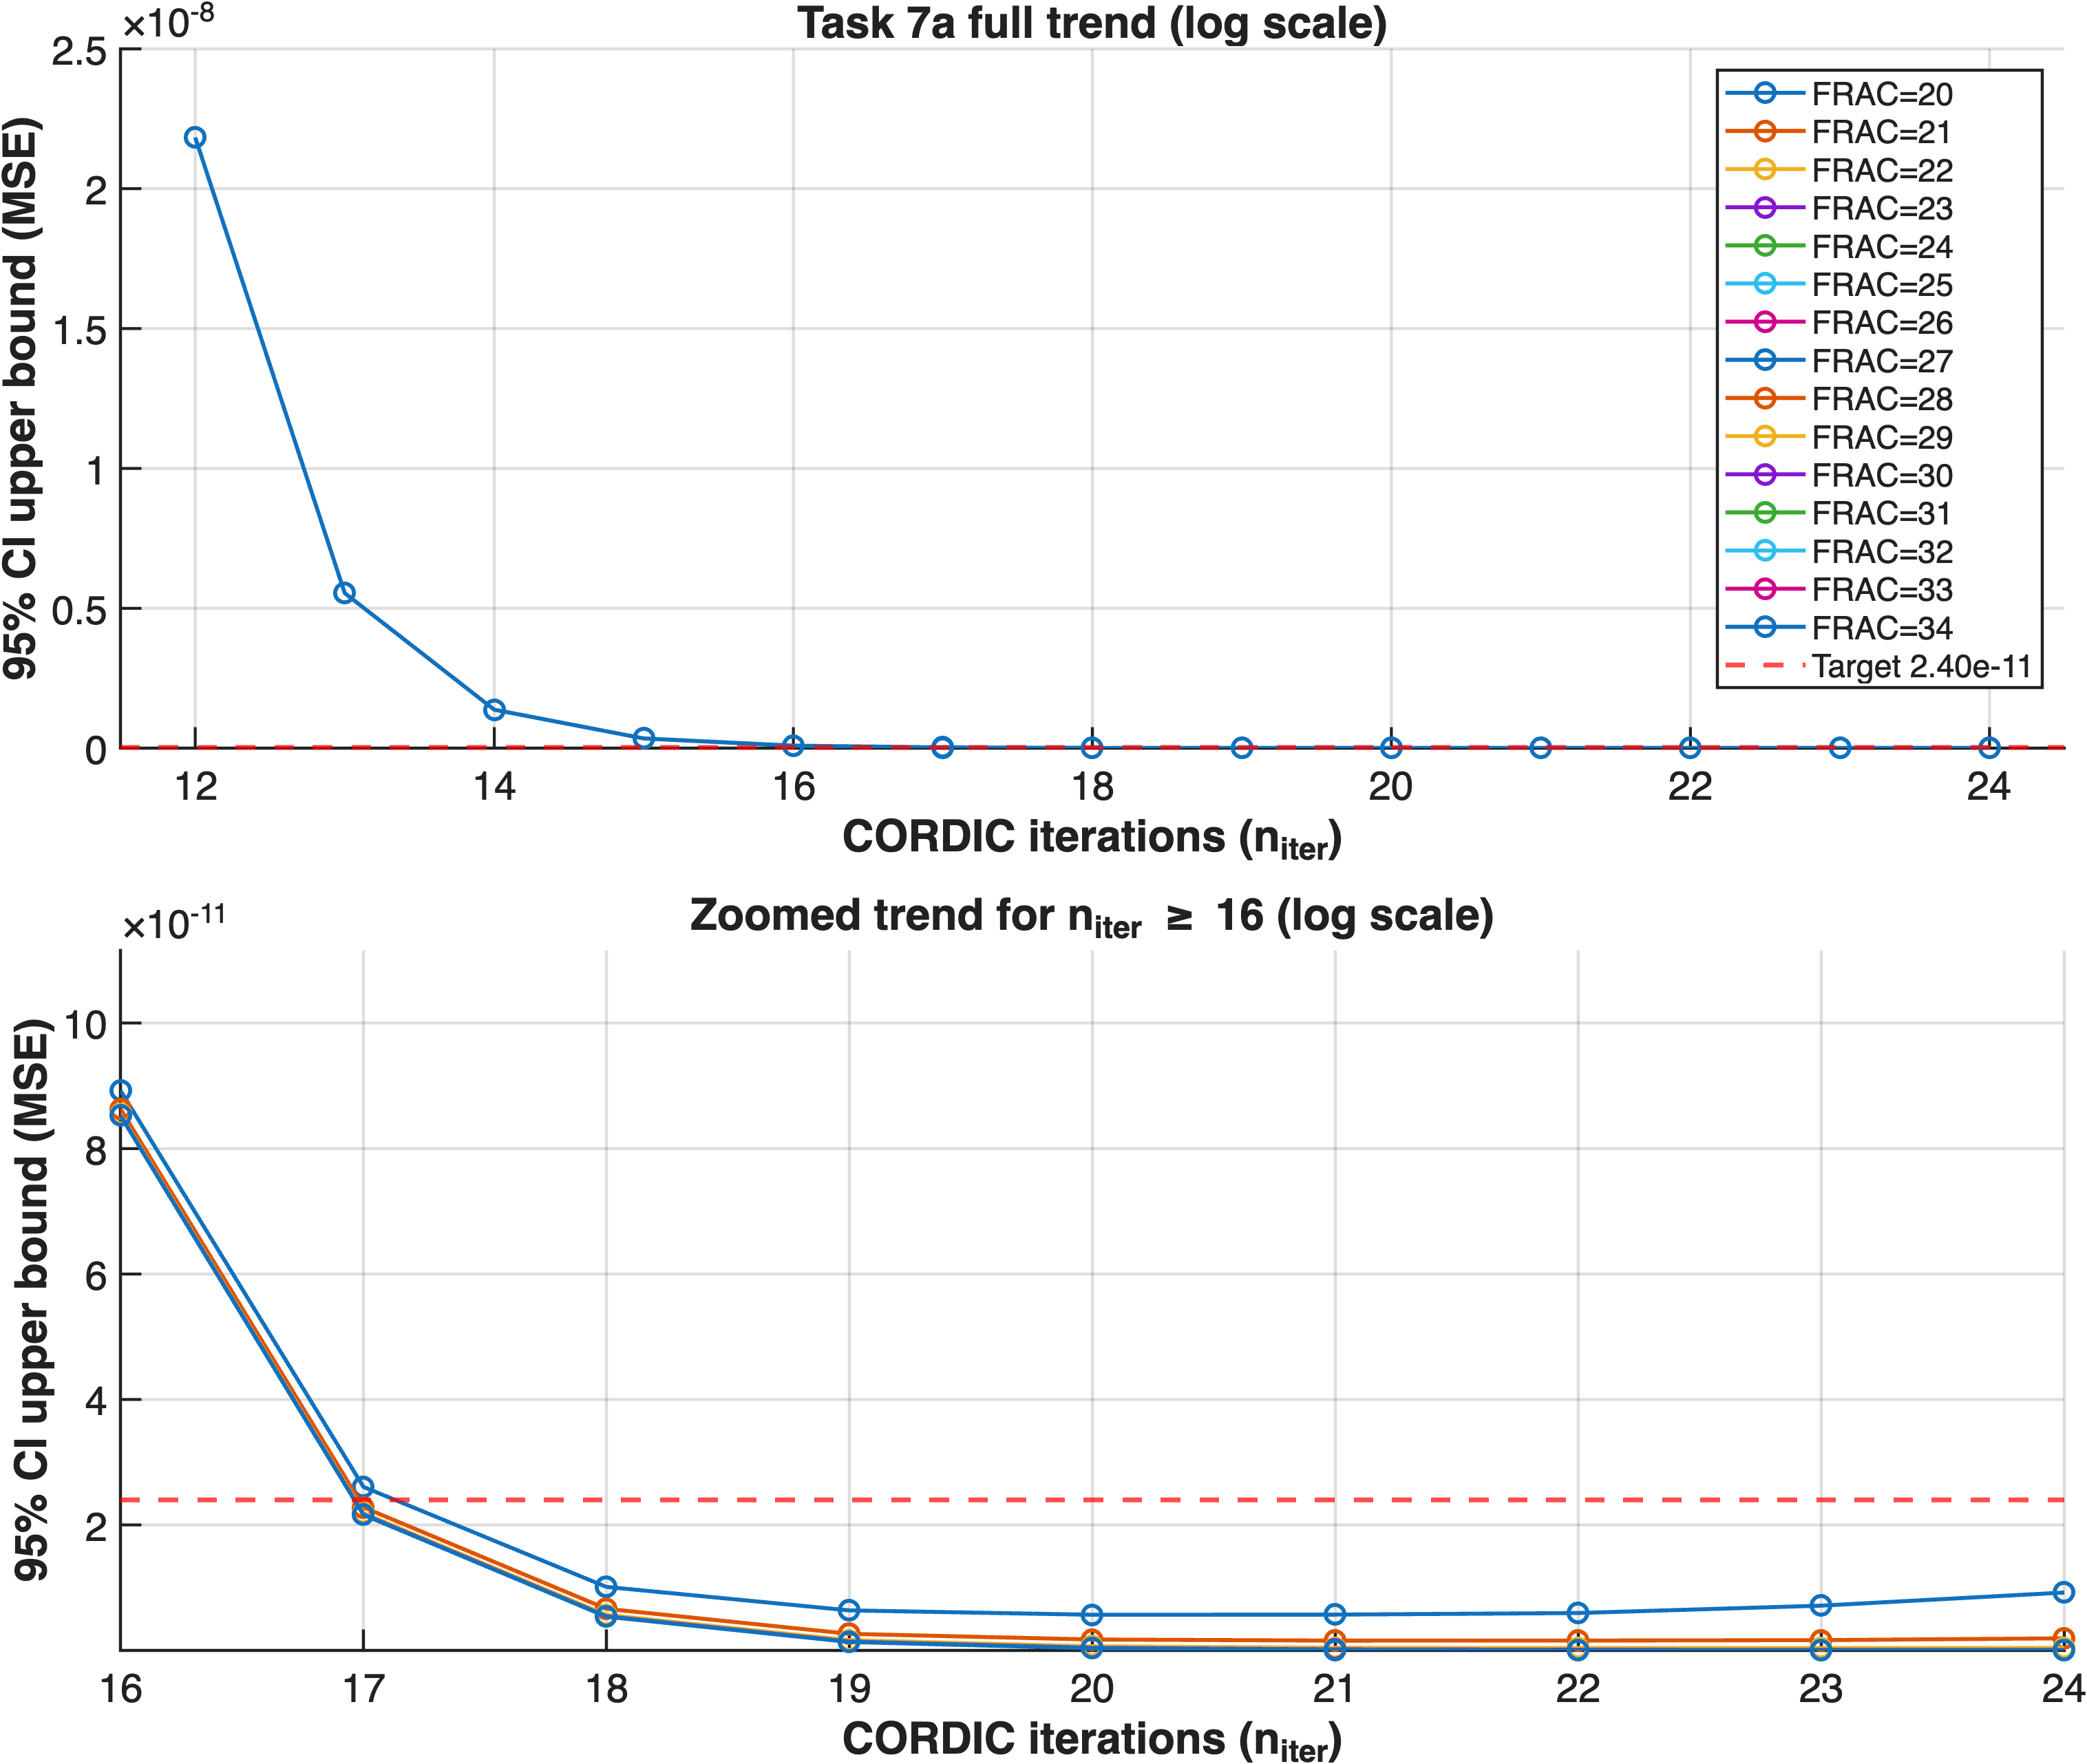
\includegraphics[width=0.98\linewidth]{Images/t7a_ci_upper_vs_iter.png}
\caption{95\% CI upper bound of MSE versus iterations for each fixed-point precision (top: full sweep; bottom: zoom for $N_{iter}\ge16$, both on log scale).}
\label{fig:t7a_ci}
\end{figure}

Figure~\ref{fig:t7a_ci} shows a clear threshold region. The error drops rapidly from 16 to 18 iterations, then flattens, which means further iterations mostly consume cycles without bringing proportionate accuracy gain for this application. Around the threshold, larger FRAC still helps, but the benefit becomes marginal once the truncation floor dominates the observed Monte Carlo error.

\begin{figure}[t]
\centering
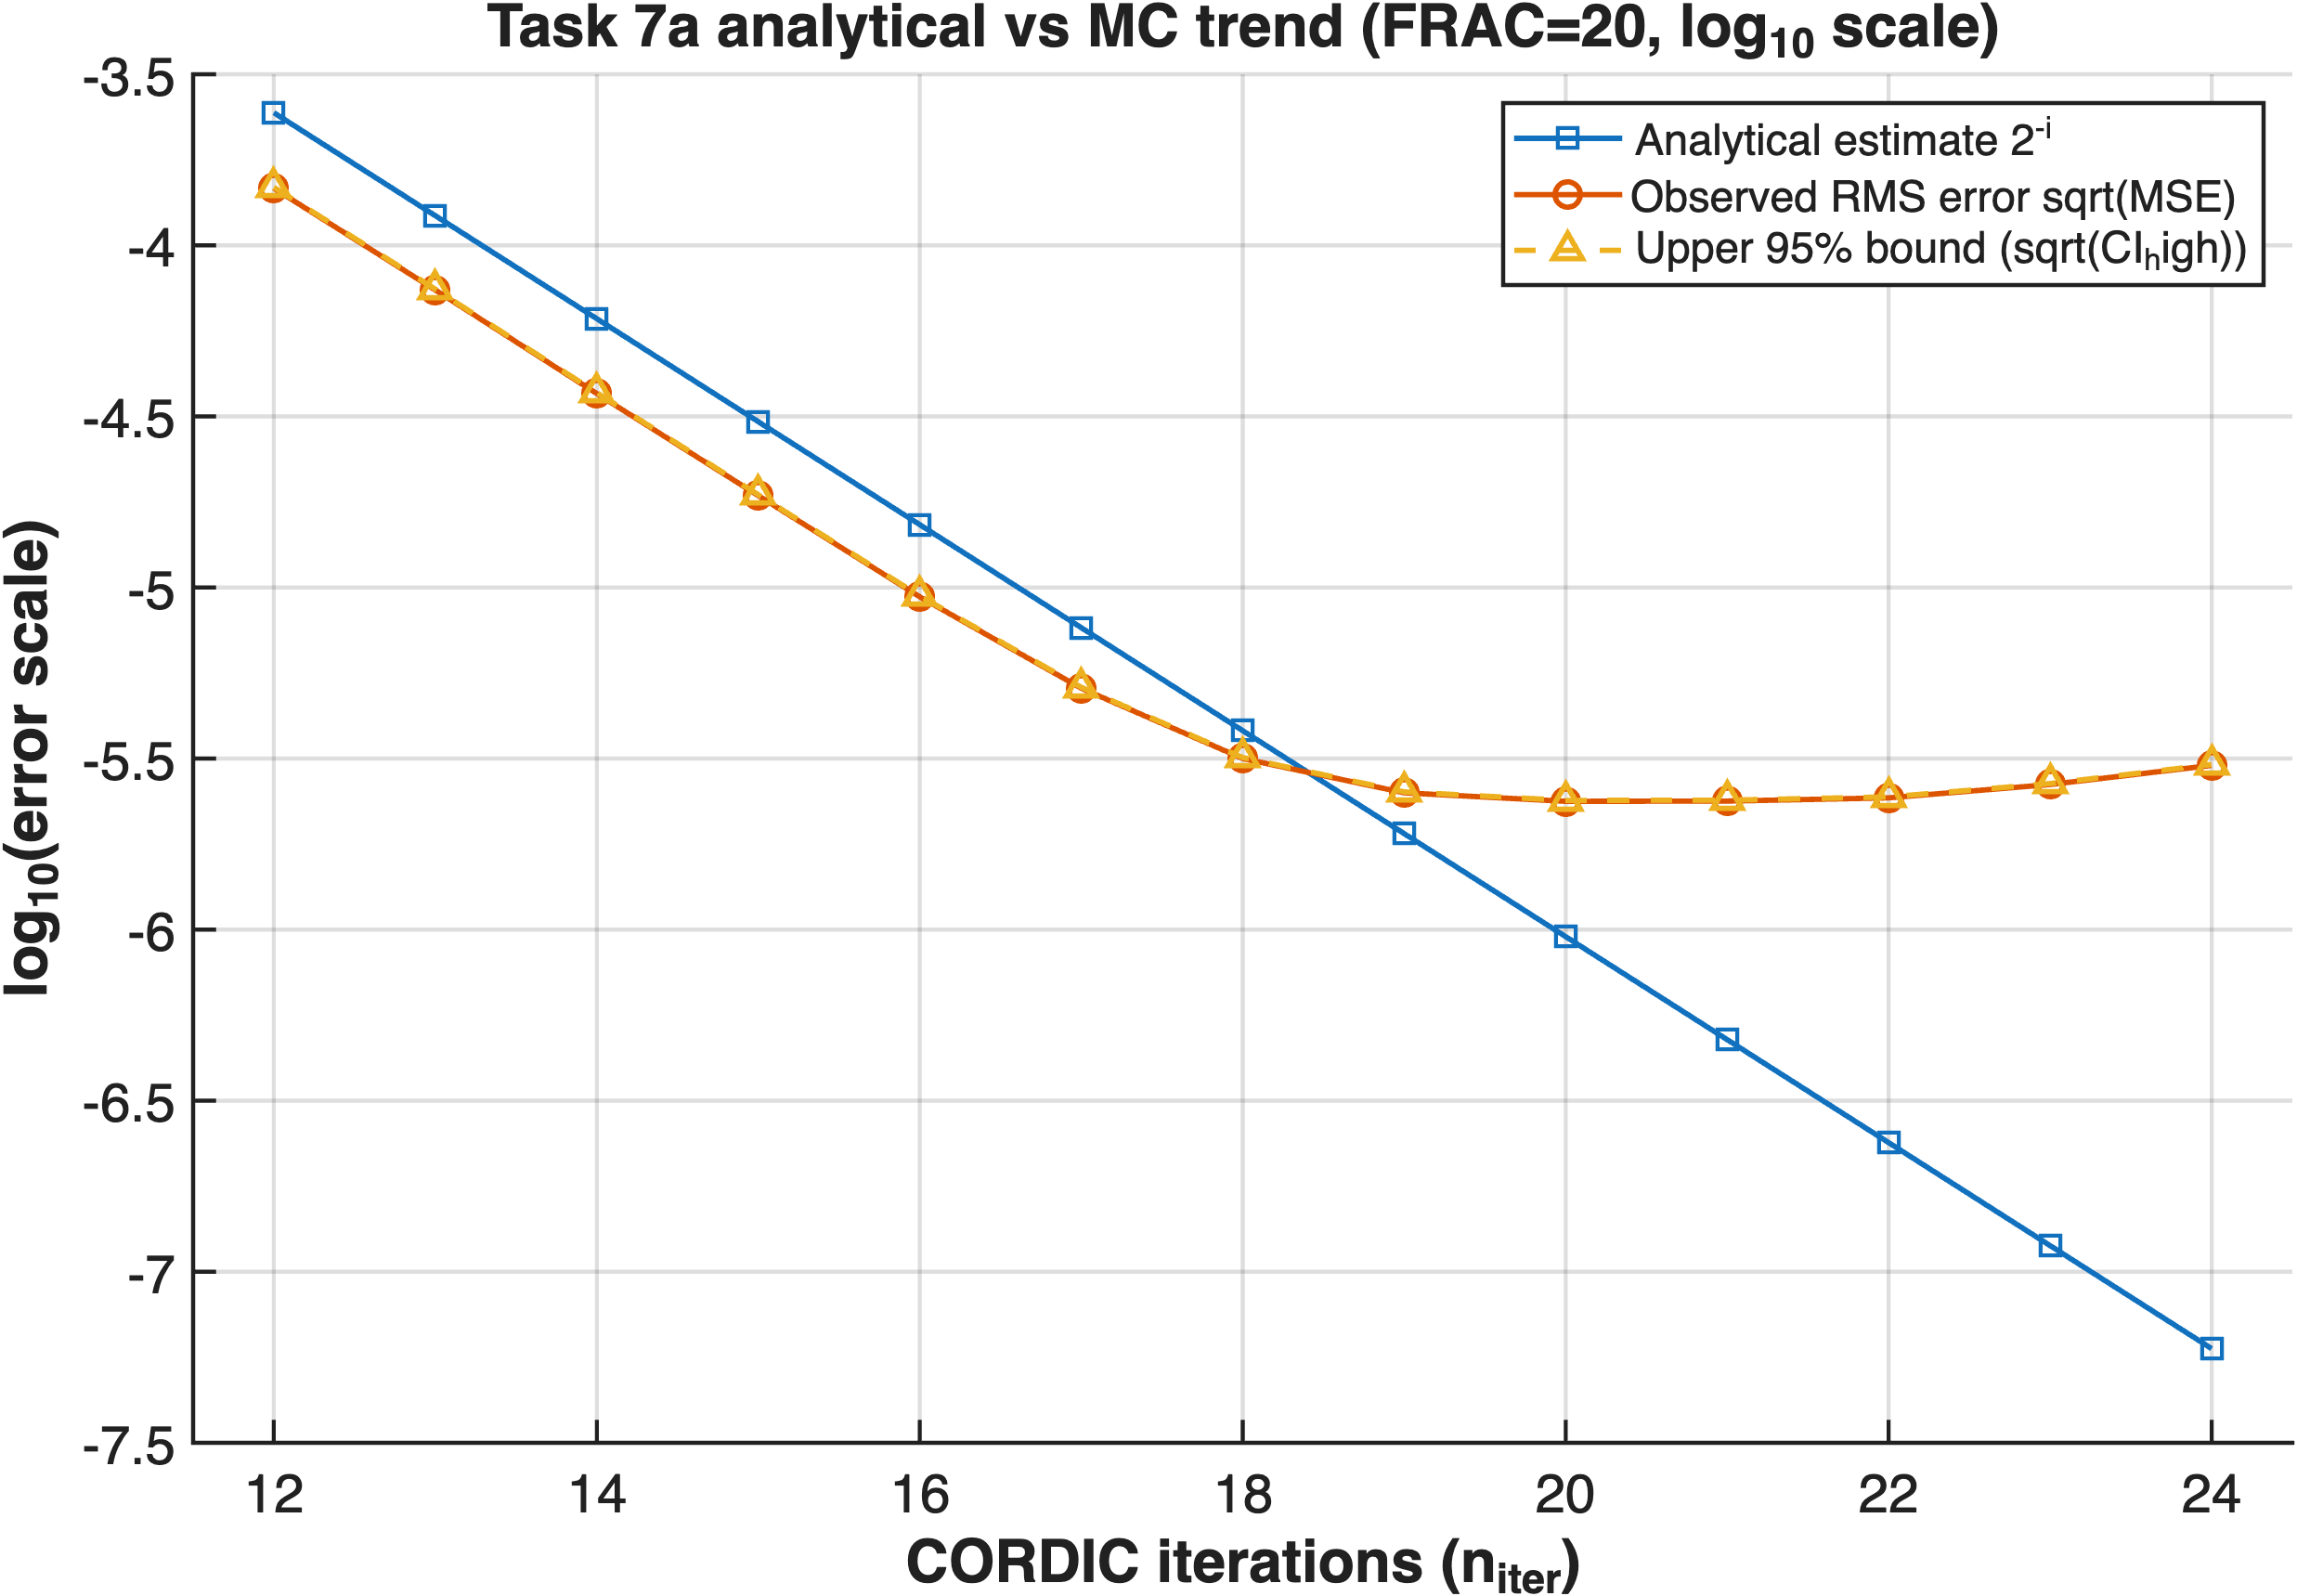
\includegraphics[width=0.98\linewidth]{Images/t7a_error_estimate_vs_mc.png}
\caption{Analytical $2^{-i}$ trend versus observed Monte Carlo error scale for FRAC$=20$ (shown in $\log_{10}$ domain).}
\label{fig:t7a_analytic_mc}
\end{figure}

The second view in Figure~\ref{fig:t7a_analytic_mc} is consistent with the design choice used later in hardware. The analytical $2^{-i}$ decay predicts the early trend well, but the measured error stops following that line once fixed-point effects dominate. This explains why the implementation does not simply maximize $N_{iter}$: after the knee point, extra iterations increase latency more reliably than they improve useful numerical accuracy.

% =============================================================
\section{Task 7b: CORDIC Architecture and Implementation}
% =============================================================

\subsection{CORDIC Microarchitecture}
The cosine block is rotation-mode fixed-point CORDIC with start/busy/done handshake. Final hardware parameters are $N_{iter}=18$, FRAC$=22$, width $W=24$, and \texttt{ITER\_PER\_CYCLE}=3, so the compute stage takes $\lceil18/3\rceil=6$ cycles; including CI issue and result-capture overhead the full handshake costs approximately 9 cycles end-to-end. Low-perturbation T7-S2 timing confirms the expected trend: for C3, the total latency is 840.1\,ms/run at \texttt{ITER\_PER\_CYCLE}=1, 828.2\,ms/run at 2, and 824.3\,ms/run at 3. The gain from 1 to 3 is therefore only about 1.9\%, which shows that software orchestration still dominates T7-S2 end-to-end runtime even though the cosine block itself becomes faster.

\begin{table}[t]
\centering
\caption{Low-perturbation T7-S2 timing versus \texttt{ITER\_PER\_CYCLE}.}
\label{tab:t7b_ipc_lp}
\footnotesize
\setlength{\tabcolsep}{3.5pt}
\begin{tabular}{lrrr}
\toprule
IPC & C2 avg (ms) & C3 avg (ms) & C4 avg (ms) \\
\midrule
1 & 26 & 840 & 29 \\
2 & 25 & 828 & 29 \\
3 & 25 & 824 & 29 \\
\bottomrule
\end{tabular}
\end{table}

\subsection{Verification and Timing}
Standalone CORDIC simulation at $\theta\in\{-1,-0.5,0,0.5,1\}$ passed with maximum absolute error $3.37\times10^{-6}$. The final build uses 3-cycle FP add/sub/mul latency (instead of the earlier 2-cycle attempt) to avoid integration mismatch. Post-fit timing remains closed at 50\,MHz (setup slack 3.106\,ns, hold slack 0.086\,ns, Fmax 59.19\,MHz).

This result also clarifies the role of \texttt{ITER\_PER\_CYCLE}. Increasing it from 1 to 3 reduces the internal CORDIC schedule from 18 cycles to 6 cycles, so it is the correct direction if the cosine engine is examined in isolation. However, the whole T7-S2 call path still spends most of its time on software-side CI dispatch and sequencing. Therefore \texttt{ITER\_PER\_CYCLE}=3 is kept because it improves the hardware block at negligible architectural cost, but is not sufficient by itself to deliver the larger system-level gain required by the marking criteria.

% =============================================================
\section{Task 7c: Single Custom Instruction Integration}
% =============================================================

\subsection{T7-S2 vs T7-S3 Integration}
T7-S2 uses separate FP\_MUL, FP\_ADD/SUB, and COS custom instructions with software scheduling. T7-S3 integrates the full inner function into one custom instruction:
\[
f(x)=0.5x + x^3\cos\left(\frac{x-128}{128}\right).
\]
The T7-S3 block reuses one FP multiplier, one FP adder, and one CORDIC core under an FSM, reducing CPU-visible calls from multiple operators per sample to one call per sample.

\subsection{Performance, Resource, and Error Results}
\begin{table}[H]
\centering
\caption{Task 7c results (avg per run, 10 runs). S/R2 = speedup vs R2-V6; S3/S2 = T7-S3 vs T7-S2.}
\label{tab:t7c_summary}
\footnotesize
\setlength{\tabcolsep}{3pt}
\begin{tabular}{lrrrrr}
\toprule
Case & T7-S2 (ms) & T7-S3 (ms) & Rel.\ err & S3/R2 & S3/S2 \\
\midrule
C2 & 25 & 7.0 & 5.0e-07 & 19.57$\times$ & 3.57$\times$ \\
C3 & 824 & 220.0 & 2.4e-05 & 19.91$\times$ & 3.75$\times$ \\
C4 & 29 & 8.0 & 2.1e-07 & 20.62$\times$ & 3.63$\times$ \\
\bottomrule
\end{tabular}
\end{table}

\begin{table}[H]
\centering
\caption{Resource/timing comparison of T7-S2 and T7-S3.}
\label{tab:t7c_resource_compare}
\footnotesize
\setlength{\tabcolsep}{3pt}
\begin{tabular}{lrr}
\toprule
Metric & T7-S2 & T7-S3 \\
\midrule
ALMs & 3767 & 3795 \\
Registers & 4207 & 4203 \\
Memory bits & 3,159,680 & 3,159,680 \\
RAM blocks & 397 & 397 \\
DSP blocks & 1 & 1 \\
Worst setup slack (ns) & 3.106 & 2.907 \\
Worst hold slack (ns) & 0.086 & 0.085 \\
Fmax \texttt{sopc\_clk} (MHz) & 59.19 & 58.5 \\
\bottomrule
\end{tabular}
\end{table}
T7-S3 adds only 28 ALMs over T7-S2 while preserving timing closure at 50\,MHz.

\begin{figure}[t]
\centering
%% Horizontal Gantt diagram.  x unit = 0.38 cm/cycle, y unit = 0.55 cm/row.
%% State boundaries (cycles): 0 1 4 7 10 13 16 17
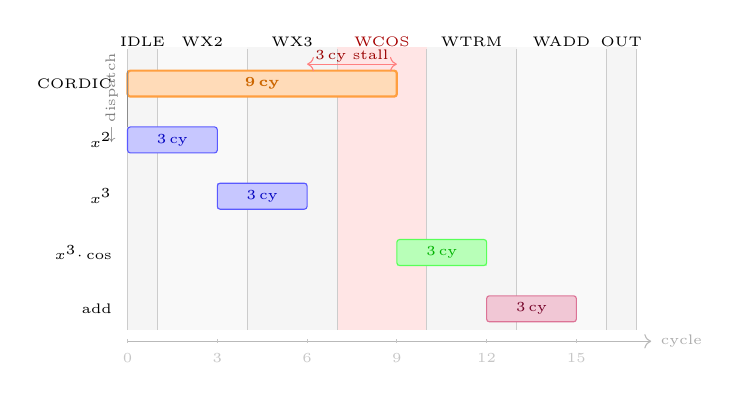
\begin{tikzpicture}[x=0.38cm, y=0.55cm, lbl/.style={font=\tiny}]
%%── State background bands ──────────────────────────────
\fill[gray!8]  (0, 0.85) rectangle (1, -5.7);
\fill[gray!5]  (1, 0.85) rectangle (4, -5.7);
\fill[gray!8]  (4, 0.85) rectangle (7, -5.7);
\fill[red!10]  (7, 0.85) rectangle (10,-5.7); %% WCOS = stall
\fill[gray!8]  (10,0.85) rectangle (13,-5.7);
\fill[gray!5]  (13,0.85) rectangle (16,-5.7);
\fill[gray!8]  (16,0.85) rectangle (17,-5.7);
%%── State boundary lines ─────────────────────────────────
\foreach \x in {0,1,4,7,10,13,16,17}
  \draw[gray!40, very thin] (\x,0.80) -- (\x,-5.7);
%%── State name labels ────────────────────────────────────
\node[lbl] at (0.5, 0.97) {IDLE};
\node[lbl] at (2.5, 0.97) {WX2};
\node[lbl] at (5.5, 0.97) {WX3};
\node[lbl, color=red!65!black] at (8.5, 0.97) {WCOS};
\node[lbl] at (11.5,0.97) {WTRM};
\node[lbl] at (14.5,0.97) {WADD};
\node[lbl] at (16.5,0.97) {OUT};
%%── Row labels ───────────────────────────────────────────
\node[lbl, anchor=east] at (-0.2,  0)    {CORDIC};
\node[lbl, anchor=east] at (-0.2, -1.3)  {$x^2$};
\node[lbl, anchor=east] at (-0.2, -2.6)  {$x^3$};
\node[lbl, anchor=east] at (-0.2, -3.9)  {$x^3{\cdot}\cos$};
\node[lbl, anchor=east] at (-0.2, -5.2)  {add};
%%── Activity bars ────────────────────────────────────────
%% CORDIC: dispatched at IDLE (t=0), 9-cycle latency
\fill[orange!28] (0,-0.30) rectangle (9, 0.30);
\draw[orange!75, thick, rounded corners=1pt] (0,-0.30) rectangle (9, 0.30);
\node[lbl, color=orange!80!black, font=\tiny\bfseries] at (4.5, 0) {9\,cy};
%% x²: dispatched simultaneously with CORDIC at IDLE (t=0), 3 cycles
\fill[blue!22] (0,-1.60) rectangle (3,-1.00);
\draw[blue!65, rounded corners=1pt] (0,-1.60) rectangle (3,-1.00);
\node[lbl, color=blue!75!black] at (1.5,-1.3) {3\,cy};
%% x³: starts after x² done (t=3), 3 cycles
\fill[blue!22] (3,-2.90) rectangle (6,-2.30);
\draw[blue!65, rounded corners=1pt] (3,-2.90) rectangle (6,-2.30);
\node[lbl, color=blue!75!black] at (4.5,-2.6) {3\,cy};
%% term (x³·cos): after CORDIC done (t=9), 3 cycles
\fill[green!28] (9,-4.20) rectangle (12,-3.60);
\draw[green!65, rounded corners=1pt] (9,-4.20) rectangle (12,-3.60);
\node[lbl, color=green!70!black] at (10.5,-3.9) {3\,cy};
%% add: after term done (t=12), 3 cycles
\fill[purple!22] (12,-5.50) rectangle (15,-4.90);
\draw[purple!55, rounded corners=1pt] (12,-5.50) rectangle (15,-4.90);
\node[lbl, color=purple!60!black] at (13.5,-5.2) {3\,cy};
%%── "Simultaneous dispatch" connector at t=0 ─────────────
%% Thin line linking left edges of CORDIC and x² bars
\draw[black!45, thin] (0, 0.30) -- (0,-1.00);
\node[lbl, color=black!50, rotate=90, anchor=south] at (0, -0.35)
     {\raisebox{0pt}{$\leftarrow$\,dispatch}};
%%── Stall annotation ─────────────────────────────────────
%% x³ finishes at t=6; CORDIC finishes at t=9: 3-cycle stall
\draw[red!50, <->, thin] (6,0.45) -- (9,0.45);
\node[lbl, color=red!60!black] at (7.5,0.63) {3\,cy stall};
%%── Cycle axis ───────────────────────────────────────────
\draw[->, gray!55, thin] (0,-5.95) -- (17.5,-5.95);
\node[lbl, right, color=gray!65] at (17.5,-5.95) {cycle};
\foreach \x in {0,3,6,9,12,15}
  \draw[gray!45,thin] (\x,-5.90) -- (\x,-6.00)
    node[below, font=\tiny]{\x};
\end{tikzpicture}
\caption{T7-S3 parallel operation (Gantt, time $\to$ right). CORDIC (orange) and $x^2$ (blue) are dispatched simultaneously at \texttt{IDLE} (left edge, marked by vertical connector). $x^3$ follows after $x^2$ completes (cycle~3). As CORDIC takes 9\,cycles vs.\ 6 for the $x^2{\to}x^3$ chain, the FSM stalls in \texttt{WCOS} (red band) for 3 extra cycles. Total: 17 FSM cycles $+{\approx}4$ Nios~II overhead $=21$.}
\label{fig:t7s3_fsm}
\end{figure}

\subsection{Latency Interpretation and HW/SW Boundary}
Isolated-cycle estimates are lower than Nios-integrated measurements. In T7-S2, one sample evaluation requires five FP multiplications, one subtraction, one addition, and one cosine call:
\[
T_{\text{T7-S2,iso}} = 5\cdot 3 + 1\cdot 3 + 1\cdot 3 + 1\cdot 9 = 30\ \text{cycles/sample}.
\]
For C3, this predicts about 39.2\,ms/run at 50\,MHz versus measured 824\,ms/run. T7-S3 isolated latency is 21 cycles. State-by-state: IDLE\,(1) $\to$ WAIT\_X2\,(3, $x^2$ computing; CORDIC starts in parallel) $\to$ WAIT\_X3\,(3, $x^3$ computing; CORDIC still running) $\to$ WAIT\_COS\,(3, waiting for CORDIC to finish; the $x^3$ path completes at cycle~6 but CORDIC takes 9 cycles matching the T7-S2 isolated cosine cost) $\to$ WAIT\_TERM\,(3, $x^3{\cdot}\cos$) $\to$ WAIT\_ADD\,(3) $\to$ OUT\,(1) = 17 FSM-state cycles, plus $\approx$4 cycles of Nios~II CI issue and result-capture overhead, totalling 21. This predicts 27.4\,ms/run idealized for C3 vs.\ measured 220.0\,ms/run. The gap confirms that software/interface overhead is the dominant term, not arithmetic depth. The theoretical floor for C3, assuming a single-cycle combinatorial f(x) CI, is $65{,}281/50\,\text{MHz} = 1.306\,\text{ms}$; the measured T7-S3 result of 220\,ms lies $168\times$ above this floor, quantifying the software-dispatch cost.

This is the central design insight governing the whole progression: the dominant variable is the hardware-software boundary placement. Operator-level CIs (T7-S2) improve individual kernels but leave software dispatch cost intact across every sample in the loop. Collapsing the entire inner function into one CI call (T7-S3) removes that per-sample overhead and is responsible for the $3.75\times$ step-up from T7-S2 to T7-S3 on C3 (low-perturbation baseline). Task~8 extends this reasoning to its logical conclusion: rather than one call per sample result, the CPU issues one PUSH per sample input and one blocking GET per frame, moving the software boundary from per-sample to per-frame granularity.

The instrumented T7-S2 run (IPC$=3$, C3) confirms this quantitatively: CI execution accounts for only 5296 of 20367 total ticks (26\%), with the remaining 74\% being software loop and dispatch overhead. Within the CI time, cosine alone contributes 775 ticks (3.8\% of total run time). This directly explains why increasing IPC yields only $\sim$1.9\% end-to-end improvement: IPC reduces cosine hardware latency by $2\times$--$3\times$, but cosine is only 3.8\% of the total, so the maximum achievable gain is bounded well below 4\%. The 74\% software overhead term is unaffected by any change inside the CI hardware.

% =============================================================
\section{Task 8: Design Progression}
% =============================================================

Three accumulator designs are explored, each moving the hardware-software boundary further from the CPU and building on the T7 arithmetic core. All close timing at 50\,MHz.

\subsection{CORDIC Consideration}
The T7 CORDIC is latency-optimised: 18 micro-rotations complete in 6 cycles (IPC=3) per evaluation, after which the next \texttt{start} can be issued. For a serialised per-sample CI call (V1) this is acceptable. For a streaming pipeline (V2), however, the iterative handshake prevents accepting a new angle while the previous cosine is in flight. V2 therefore replaces the FSM with an 18-stage fully pipelined register chain (\texttt{task8\_cordic\_cos\_pipe}), accepting one new angle per cycle after 18-cycle fill. Parameters $N_{iter}{=}18$, $W{=}24$ are retained: pipeline depth adds fill latency but does not reduce steady-state throughput, so the T7a accuracy margin is preserved without extra cost.

Two further optimisations are noted but not implemented due to time constraint. First, the T7a sweep shows that $N_{iter}=17$ already satisfies the acceptance criterion at FRAC$=21$; reducing pipeline depth to 17 stages would shrink fill latency by 1 cycle and save 1 register stage of area, with no steady-state throughput penalty. For C3 ($N=65{,}281$), the 18-cycle fill represents $18/65{,}281 < 0.03\%$ overhead, so the gain is mainly area rather than performance. Second, the fixed-point width $W=24$ used in the pipeline is uniform across all 18 stages. Later iterations rotate by $2^{-i}$, contributing progressively less to the final result, so a tapered-width implementation (narrowing $W$ with $i$) could reduce register area further. Both optimisations are straightforward extensions within the same architectural framework.

\subsection{V1: Stateless Accumulate CI}
\texttt{task8\_ci\_f2\_accum} takes \texttt{(acc\_in,\,x)} and returns \texttt{acc\_in\,+\,f(x)} with no internal running sum. It reuses the T7-S3 f(x) FSM and appends one FP addition stage: 17 FSM cycles $+$ 3 (extra FP add) $= 20$ FSM cycles, plus ${\approx}4$ Nios overhead $= 24$ cycles per sample. Software initialises \texttt{acc\,=\,0} and calls \texttt{CI(acc,\,x[i])} in a tight loop, which accepts current sum, returns updated sum.

\begin{table}[H]
\centering
\caption{T8-V1 on-board results (10 runs, 1\,kHz; C1 excluded (below timer resolution and elevated numerical error)).}
\label{tab:t8v1_results}
\footnotesize
\setlength{\tabcolsep}{2.4pt}
\begin{tabular}{lrrrr}
\toprule
Case & Lat.(ms) & Rel.err & S/R2-V6 & S/T7-S3 \\
\midrule
C2 & 4 & 8.1e-07 & 34.25$\times$ & 1.75$\times$ \\
C3 & 133 & 1.7e-05 & 32.93$\times$ & 1.65$\times$ \\
C4 & 4 & 1.3e-06 & 41.25$\times$ & 2.00$\times$ \\
\bottomrule
\end{tabular}
\end{table}

Resource footprint matches T7-S3 closely: ALMs\,3793, Reg\,4214, DSP\,1, setup slack\,3.205\,ns, Fmax\,59.54\,MHz. The marginal gain over T7-S3 ($1.65\text{--}2.00\times$) confirms that collapsing the final accumulate into the CI call removes one round-trip but leaves per-sample dispatch overhead otherwise unchanged.

\subsection{V2: Fully Pipelined Streaming CI}
V2 targets one $f(x)$ per cycle by replacing the per-sample CI call with a PUSH-based protocol. The core chains round-robin FP stages (LANES$=6$) through the datapath
\begin{align*}
x &\;\to\; x^2 \;\to\; x^3 \;\xrightarrow{\text{FIFO}}\; x^3{\cdot}\cos\!\left(\tfrac{x-128}{128}\right) \\
 &\;\to\; f(x) \;\to\; \text{accumulate}
\end{align*}
A 32-entry FIFO bridges the 18-cycle CORDIC pipeline against the 12-cycle $x{\to}x^3$ path ($x^2$ then $x^3$, each 6 cycles). The interleaved accumulator (ACC\_LANES$=6$) distributes partial sums across 6 independent lanes to break the FP-add loop-carried dependency. The CI front-end (\texttt{task8\_ci\_fsum\_pipe}) exposes INIT/PUSH\_X/GET\_RESULT opcodes; \texttt{PUSH\_X} returns immediately so the CPU issues the next sample before the previous exits the pipeline. The Nios driver calls \texttt{CI(INIT,\,N)} once, then loops \texttt{CI(PUSH\_X,\,x[i])} for $i=0\ldots N{-}1$ with no blocking, and finally calls \texttt{CI(GET\_RESULT,\,0)} which stalls until the pipeline drains and returns $F(X)$.

\begin{figure}[t]
\centering
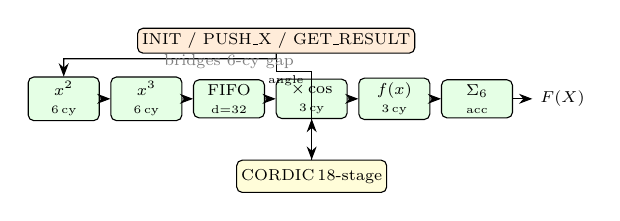
\begin{tikzpicture}[scale=0.82, every node/.append style={transform shape},
  blk/.style={draw, rounded corners=2pt, font=\scriptsize, inner sep=2pt, align=center,
              minimum width=1.1cm, minimum height=0.5cm, fill=green!10},
  ci/.style ={draw, rounded corners=2pt, font=\scriptsize, inner sep=2pt,
              minimum width=3.6cm, minimum height=0.37cm, fill=orange!15},
  cord/.style={draw, rounded corners=2pt, font=\scriptsize, inner sep=2pt, align=center,
               minimum width=2.0cm, minimum height=0.5cm, fill=yellow!15},
  arr/.style={->, >=Stealth, thin},
  lbl/.style={font=\tiny},
]
% Pipeline nodes (x2..acc spaced at 1.1+0.18=1.28cm)
\node[ci]   at (3.84, 0)    (ci)   {INIT / PUSH\_X / GET\_RESULT};
\node[blk]  at (0.55,-0.9)  (x2)   {$x^2$\\\tiny 6\,cy};
\node[blk]  at (1.83,-0.9)  (x3)   {$x^3$\\\tiny 6\,cy};
\node[blk]  at (3.11,-0.9)  (fifo) {FIFO\\\tiny d=32};
\node[blk]  at (4.39,-0.9)  (term) {${\times}\cos$\\\tiny 3\,cy};
\node[blk]  at (5.67,-0.9)  (fx)   {$f(x)$\\\tiny 3\,cy};
\node[blk]  at (6.95,-0.9)  (acc)  {$\Sigma_6$\\\tiny acc};
\node[cord] at (4.39,-2.1)  (cord) {CORDIC\,18-stage};
% Arrows
\draw[arr] (ci) -- ++(0,-0.28) -| (x2.north);
\draw[arr] (ci.south) -- ++(0,-0.28) -| (cord.north)
           node[lbl,pos=0.55,left]{\tiny angle};
\draw[arr] (x2) -- (x3);  \draw[arr] (x3) -- (fifo);
\draw[arr] (fifo) -- (term);  \draw[arr] (term) -- (fx);
\draw[arr] (fx)   -- (acc);
\draw[arr] (cord.north) |- (term.south);
\draw[arr] (acc.east) -- ++(0.3,0) node[right,font=\scriptsize]{$F(X)$};
\node[lbl,color=gray,above=1pt of fifo]{\scriptsize bridges 6-cy gap};
\end{tikzpicture}
\caption{T8-V2 pipeline. Input $x$ feeds the $x^2{\to}x^3$ top path and the CORDIC angle path; FIFO-32 absorbs the latency mismatch; round-robin FP lanes sustain one output per cycle.}
\label{fig:t8v2_pipe}
\end{figure}

\begin{table}[H]
\centering
\caption{T8-V2 on-board results (10 runs, 1\,kHz).}
\label{tab:t8v2_results}
\footnotesize
\setlength{\tabcolsep}{2.4pt}
\begin{tabular}{lrrrr}
\toprule
Case & Lat.(ms) & Rel.err & S/R2-V6 & S/T7-S3 \\
\midrule
C2 & 2 & 1.2e-06 & 68.50$\times$ & 3.50$\times$ \\
C3 & 75 & 2.9e-05 & 58.40$\times$ & 2.93$\times$ \\
C4 & 2 & 1.1e-06 & 82.50$\times$ & 4.00$\times$ \\
\bottomrule
\end{tabular}
\end{table}

V2 correctness is verified across all cases. Resource cost is substantially higher than V1: ALMs\,13{,}955 (44\%), Reg\,29{,}723, DSP\,18, RAM\,397/397 (100\%). The increase reflects 6 round-robin MUL lanes, 6 ADD lanes, and the 18-stage CORDIC pipeline operating in parallel.

\textbf{Pipeline utilisation.} The whole datapath from $x$ to accumulate spans roughly 26 clock cycles (18-stage CORDIC + 6 MUL/ADD stages + FIFO bridging). For C3 ($N=65{,}281$), fill-drain overhead is $26/65{,}281 < 0.04\%$, giving effective utilisation $>99.9\%$. Even for C2 ($N=2{,}041$), fill overhead is $26/2{,}041 \approx 1.3\%$, so the pipeline is essentially fully loaded for all evaluated cases. The throughput gain over V1 is $1.77\text{--}2.00\times$ on C3/C2/C4; the modest ratio indicates that the Nios PUSH\_X dispatch loop remains the limiting factor, not the pipeline throughput itself.

\subsection{V3: Memory-Mapped DMA Interface (analysis)}
V3 (\texttt{task8\_mm\_fsum\_accel}) moves the hardware-software boundary to the frame level: the Nios processor writes the frame length, asserts START via Avalon-MM CSR, launches a single mSGDMA descriptor to stream the input array into the accelerator's Avalon-ST sink, then polls DONE. No per-sample CPU interaction occurs. The arithmetic core reuses the T7-S3 iterative f(x) block, so per-sample latency is unchanged from V1; the gain is the complete elimination of CI dispatch overhead for all $N$ samples in one DMA transfer. RTL functional simulation passes, confirming the datapath logic is correct. However, completing the on-board integration requires Platform Designer component wiring (mSGDMA + custom accelerator), BSP regeneration, and software driver bring-up; this was not achieved within the available time.

% =============================================================
\section{Cross-Task Comparison}
% =============================================================

\begin{table}[H]
\centering
\caption{Cross-stage comparison against the R2-V6 baseline.}
\label{tab:cross_task_compare}
\footnotesize
\setlength{\tabcolsep}{2.0pt}
\begin{tabular}{lrrrrrr}
\toprule
Stage & C2(ms) & C3(ms) & C4(ms) & ALMs & DSP & C3 S/R2-V6 \\
\midrule
R2-V6 & 137.0 & 4380.0 & 165.0 & 2103 & 6 & 1.00$\times$ \\
T7-S2 & 25 & 824 & 29 & 3767 & 1 & 5.32$\times$ \\
T7-S3 & 7.0 & 220.0 & 8.0 & 3795 & 1 & 19.91$\times$ \\
T8-V1 & 4 & 133 & 4 & 3793 & 1 & 32.93$\times$ \\
T8-V2 & 2 & 75 & 2 & 13955 & 18 & 58.40$\times$ \\
\bottomrule
\end{tabular}
\end{table}

\begin{figure}[H]
\centering
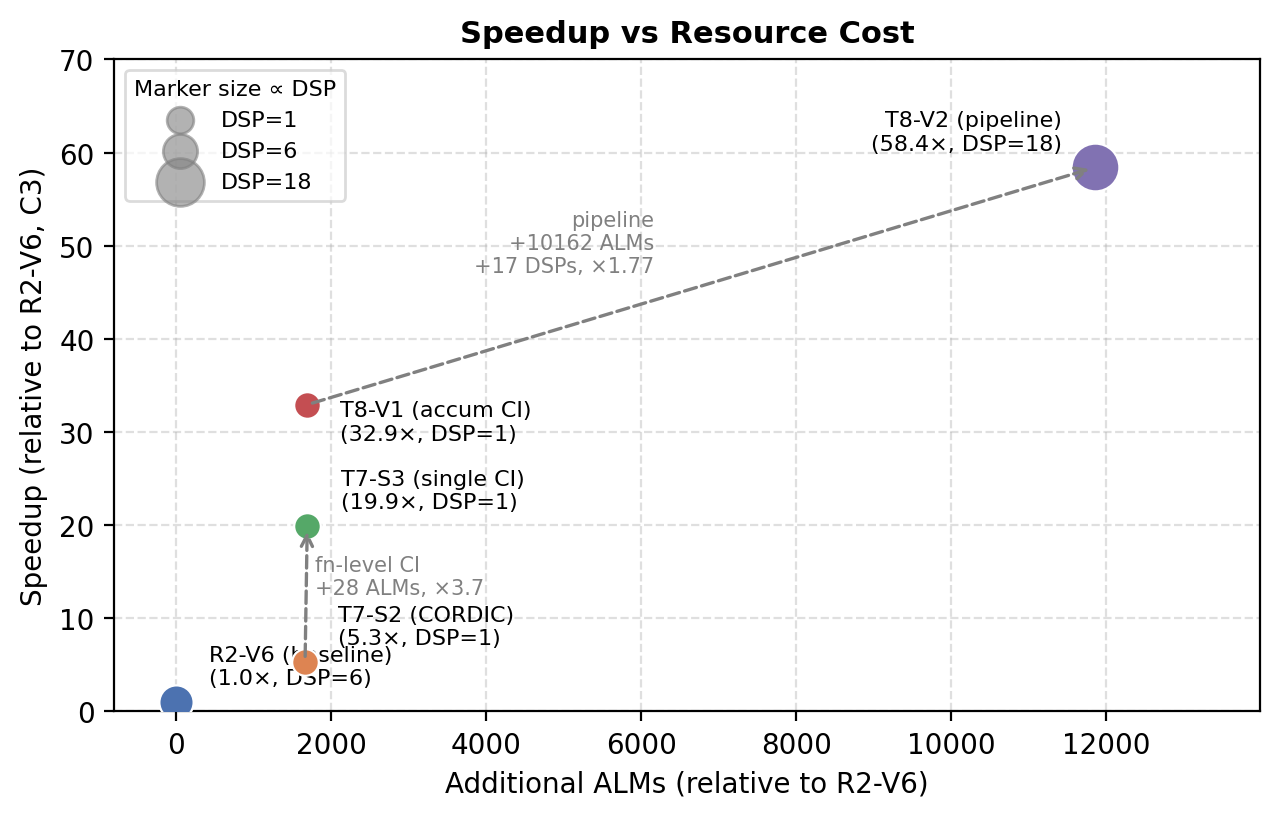
\includegraphics[width=0.98\linewidth]{Images/r3_speedup_alms.png}
\caption{Speedup vs.\ additional ALM cost relative to R2-V6. T7-S2, T7-S3 and T8-V1 lie at nearly the same ALM count, showing that interface-level decisions dominate performance gains in that region.}
\label{fig:speedup_alms}
\end{figure}

Table~\ref{tab:cross_task_compare} shows a clear progression. T7-S2 gains $5.32\times$ over R2-V6 by replacing software \texttt{cosf} with CORDIC (low-perturbation), but per-sample dispatch still dominates. T7-S3 collapses the inner arithmetic chain into one CI call per sample, reaching $19.91\times$ on C3 with correctness verified. T8-V1 reduces latency further by folding the accumulate step into the CI itself ($32.93\times$ on C3, correctness verified). T8-V2 deploys the fully pipelined streaming design, reaching $58.40\times$ on C3 (correctness verified) at the cost of a larger resource footprint (ALMs\,13{,}955, DSP\,18). The jump from T7-S3 to T8-V2 confirms that the hardware-software boundary is the dominant design variable: moving from per-sample CI calls to a pipelined PUSH protocol delivers an additional $2.93\times$ even though the Nios PUSH loop is still the steady-state bottleneck.

% =============================================================
\section{What I Would Do Differently}
% =============================================================

Accumulating in fp32 introduces a rounding floor that grows with $N$; for C3 ($N=65{,}281$) this is already visible in the rel.err figures. A single fp64 running sum (with fp32 inputs and outputs) would suppress this growth at the cost of one wider adder, a negligible resource overhead given the available ALMs.

The T8-V2 FIFO depth of 32 was chosen empirically; analytically, the minimum is $18-12=6$ cycles (CORDIC minus $x{\to}x^3$ path latency), so depth 32 is over-provisioned. The T7a sweep also shows $N_{iter}=17$ already satisfies the accuracy criterion, yet T8 reuses $N_{iter}=18$ without re-evaluation, adding 1 redundant pipeline stage.

Most importantly, V2 and V3 should have been merged: attaching the V2 fully pipelined core to the V3 Avalon-ST interface would let mSGDMA feed one sample per cycle with no CPU involvement, approaching the 1.306\,ms ideal floor that V2 cannot reach because the PUSH\_X loop is still the bottleneck.

The 1\,kHz tick source limits timing resolution to 1\,ms per tick, making C1 ($N=52$) and small-$N$ cases unreliable and forcing C1 to be excluded from comparison tables. Replacing the tick counter with a higher-resolution hardware timer (e.g.\ the Nios~II performance counter at 50\,MHz) would allow accurate timing of sub-millisecond cases.

% =============================================================
\section{Conclusions}
% =============================================================

The validated progression links three design decisions: Task~7a selects a defensible CORDIC operating point ($N_{iter}=18$, $W=24$, FRAC$=22$), Task~7b validates the CORDIC microarchitecture at IPC$=3$ (confirming timing closure and bounding the cosine contribution to 3.8\% of runtime), and Task~7c achieves the largest single gain ($19.91\times$ on C3) by collapsing the inner arithmetic sequence into one CI call per sample. Task~8-V1 folds the accumulate step into the CI call ($32.93\times$ on C3); T8-V2 deploys a fully pipelined CORDIC with round-robin FP stages and an interleaved accumulator, reaching $58.40\times$ on C3 at the cost of a larger resource footprint (ALMs\,13{,}955, DSP\,18). A third design (T8-V3) targets the frame-level boundary via Avalon-MM + DMA; RTL simulation passes but board integration is incomplete. The dominant design variable throughout is the hardware-software boundary: operator-level CIs improve individual kernels but leave software dispatch dominant, while function-level and then streaming interfaces progressively remove that overhead.

\FloatBarrier
\end{document}
